\chapter{Jim Rohn -- GSI Master Trainer Seminar 2003}

This lecture begins with a small number and ends with a philosophy. Rohn does not start by telling us to dream bigger; he starts by asking what, in practical economic terms, could possibly move a worker from a low wage toward a different future. From there he builds, in order, a sequence of rejected strategies, a ladder of repeated multiplication, a rule of self-development, a theory of language, a ladder of widening productivity, a few old ratio laws, and finally a picture of personal philosophy as a guidance system. The gain in these notes is not to make the lecture sound more technical than it is, but to let its arithmetic and structure stand out clearly.

\begin{remark}
These notes follow a Jim Rohn original talk from a curated playlist rather than a formal institutional course. The transcript is the primary source, and the present chapter is organized through the Video2Book workflow associated with LazyingArt LLC. No validated lecture screenshots survive for this chapter, so every displayed equation and every diagram below is a cautious transcript-derived reconstruction rather than a transcription of visible board work.
\end{remark}

\section{Economic Philosophies and the Turn to Performance}

The opening transcript line is garbled, but the practical setup is stable. We are at the low end of the wage scale, around \(\$5\) an hour, and the question is: how does such a wage change? Rohn does not answer immediately. Instead, he stages three familiar responses and lets their limitations appear.

The first philosophy is to wait for government to change the minimum wage. The second is to wait for the company to decide to pay more. The third is to demand more money, especially if one is not alone but part of a group large enough to apply pressure. The lecture is careful here. Demand is not said to be meaningless. Together with others, it may produce a little movement. But it does not yet solve the real problem.

At the opening of the lecture, then, the stable numbers are
\begin{equation}
w_0=\$5/\text{hour}, \qquad w_1=\$6/\text{hour}.
\end{equation}
That is the scale of the initial discussion. We are not yet at wealth; we are at the first dollar of movement.

The philosophy Rohn finally keeps is performance. He says, in effect: I will perform so well that it becomes embarrassing not to pay me more. As a compact shorthand for his spoken sequence of examples, we may write
\begin{equation}
\$5/\text{hour}\to \$6/\text{hour}\to \$8/\text{hour}\to \$10/\text{hour}\to \$20/\text{hour}.
\end{equation}
This is not a board transcription. It is a faithful compression of the lecture's spoken escalation.

\begin{figure}[t]
\centering
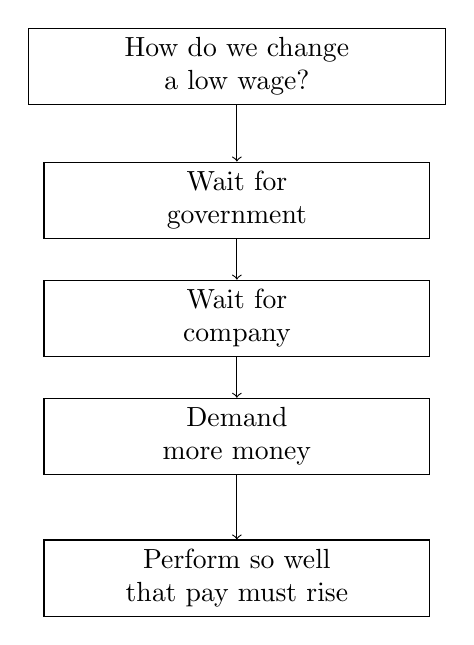
\begin{tikzpicture}[x=1cm,y=1cm]
\node[draw, rectangle, align=center, minimum width=5.3cm, minimum height=0.9cm] (top) at (0,0) {How do we change\\a low wage?};
\node[draw, rectangle, align=center, minimum width=4.9cm, minimum height=0.8cm] (g) at (0,-1.7) {Wait for\\government};
\node[draw, rectangle, align=center, minimum width=4.9cm, minimum height=0.8cm] (c) at (0,-3.2) {Wait for\\company};
\node[draw, rectangle, align=center, minimum width=4.9cm, minimum height=0.8cm] (d) at (0,-4.7) {Demand\\more money};
\node[draw, rectangle, align=center, minimum width=4.9cm, minimum height=0.9cm] (p) at (0,-6.5) {Perform so well\\that pay must rise};
\draw[->] (top) -- (g);
\draw[->] (g) -- (c);
\draw[->] (c) -- (d);
\draw[->] (d) -- (p);
\end{tikzpicture}
\caption{Transcript-derived reconstruction of the lecture's opening logic. The decisive move is not simply to ask harder, but to become more valuable.}
\end{figure}

The importance of this turn is easy to miss if we summarize too quickly. Rohn is not merely adding a fourth slogan to the first three. He is rejecting three ways of thinking and keeping one. That is why he immediately says that if we wish to change our economic future, it starts with personal philosophy.

\subsection{Question \& Answer}

\paragraph{Question.} Why can demand produce some progress and yet still fail as a path to wealth?

\paragraph{Answer.} Because demand acts from the outside. It may alter the employer's decision at one point. But performance acts from the inside: it changes what sort of worker we are, and therefore what scale of compensation becomes reasonable. A collective demand may get us from \(5\) to \(6\). It does not yet explain how one climbs an entire ladder.

That is the point of the opening elimination. Once the weak philosophies are set aside, the lecture can ask a much larger question.

\section{The Income-Multiplication Ladder}

Now Rohn broadens the horizon. If one can think of somebody making \(\$5\) an hour, and also somebody making \(\$50\) an hour, then one arithmetic fact is already in front of us:
\begin{equation}
w \mapsto 10w.
\end{equation}
This is the lecture's first genuine mathematical spine. It is elementary arithmetic, but it is not used trivially. It is used pedagogically. Rohn wants the audience to learn to ask, in sequence, whether the same operation can happen again.

As note-writer shorthand, we may organize the repeated question by the recursion
\begin{equation}
w_{k+1}=10w_k.
\end{equation}
With \(w_0=\$5/\text{hour}\), the lecture's ladder becomes
\begin{align}
w_0 &= \$5/\text{hour}, \\
w_1 &= 10w_0 = \$50/\text{hour}, \\
w_2 &= 10w_1 = \$500/\text{hour}, \\
w_3 &= 10w_2 = \$5{,}000/\text{hour}, \\
w_4 &= 10w_3 = \$50{,}000/\text{hour}.
\end{align}
The lecture's force lies in the repetition of the question: if it is possible once, would it be possible again? And again? Each rung is made socially plausible by an example. A Beverly Hills lawyer supplies the \(\$500\) rung. The speaker playfully places himself near the \(\$5{,}000\) rung. General Schwarzkopf, at about
\begin{equation}
w_{\mathrm{speech}}\approx \$65{,}000/\text{hour},
\end{equation}
shows that even the upper end of the sequence is not merely fantasy.

\begin{figure}[t]
\centering
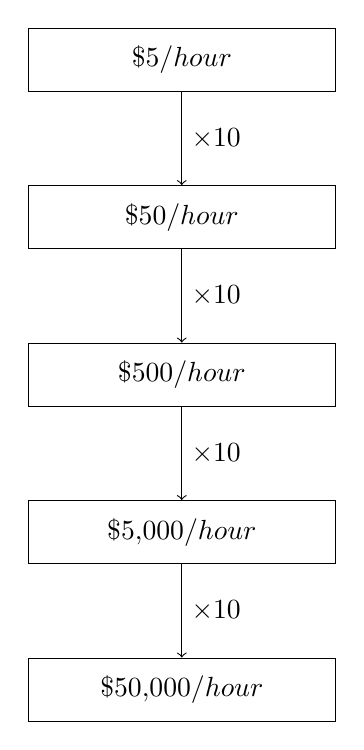
\begin{tikzpicture}[x=1cm,y=1cm]
\node[draw, rectangle, align=center, minimum width=3.9cm, minimum height=0.8cm] (a) at (0,0) {\(\$5/\text{hour}\)};
\node[draw, rectangle, align=center, minimum width=3.9cm, minimum height=0.8cm] (b) at (0,-2.0) {\(\$50/\text{hour}\)};
\node[draw, rectangle, align=center, minimum width=3.9cm, minimum height=0.8cm] (c) at (0,-4.0) {\(\$500/\text{hour}\)};
\node[draw, rectangle, align=center, minimum width=3.9cm, minimum height=0.8cm] (d) at (0,-6.0) {\(\$5{,}000/\text{hour}\)};
\node[draw, rectangle, align=center, minimum width=3.9cm, minimum height=0.8cm] (e) at (0,-8.0) {\(\$50{,}000/\text{hour}\)};
\draw[->] (a) -- node[right] {\(\times 10\)} (b);
\draw[->] (b) -- node[right] {\(\times 10\)} (c);
\draw[->] (c) -- node[right] {\(\times 10\)} (d);
\draw[->] (d) -- node[right] {\(\times 10\)} (e);
\end{tikzpicture}
\caption{A narrow reconstruction of the lecture's repeated tenfold ladder. The point is not a formal growth law but a sequence of increasingly ambitious questions.}
\end{figure}

Rohn also inserts a yearly anchor: one person earned about
\begin{equation}
Y_{\text{one year}}\approx \$63\,\text{million}.
\end{equation}
This is not analyzed any further. It is there to stretch the sense of scale before he gives the operative rule for climbing.

\subsection{Question \& Answer}

\paragraph{Question.} If income can multiply by ten once, why not again?

\paragraph{Answer.} Arithmetically, there is no obstacle. Once the first jump is admitted, nothing in the operation \(w\mapsto 10w\) forbids the next jump. The real obstacle is elsewhere. It lies in what sort of person, skill, discipline, and value would make a higher rung occupiable.

That last sentence is the hinge of the chapter. The lecture has now enlarged the number. It is ready to tell us what enlarges the person.

\section{Success, Person-Formation, and the Extraordinary Life}

Rohn's answer to the question of ascent is brief enough to sound almost too simple. That simplicity is deceptive. He says: learn to work harder on yourself than you do on your job. The lecture has asked how we climb the arithmetic ladder; now it answers with a principle of self-construction.

We may compress his contrast into the following pair:
\begin{equation}
\text{hard work on the job} \to \text{a living}, \qquad
\text{hard work on oneself} \to \text{a fortune}.
\end{equation}
This is not his formal notation, but it is his explicit distinction. He says that once he understood this philosophy, it changed his life. The income ladder, which could have remained mere provocation, is now supplied with a mechanism.

That mechanism is not a technique alone. It is a change of person. Hence the lecture's next famous sentence:
\begin{equation}
\text{success} \approx \text{attraction}(\text{the person one becomes}).
\end{equation}
Rohn states it negatively as well as positively: success is not something we pursue; it is something we attract by becoming an attractive person. This is the shift from arithmetic to anthropology. The money matters, but the money follows the becoming.

The same movement appears when he broadens the target beyond earnings. He says, slowly and repeatedly, that from testimonials and from personal experience we have enough information to conclude that it is possible to design and build and live an extraordinary life. We should not rush past that sentence. It is the lecture's attempt to move from isolated success stories to a general existential possibility.

What changes at this point is the scale of the question. We began with \(\$5\) and \(\$6\). We are now asking whether a life itself can be deliberately designed. But Rohn does not leave that claim floating in abstraction. He situates it historically.

\section{The Twenty-First Century: Opportunity, Competition, Mind, and Words}

The lecture now shifts from private development to public time. Rohn's claim is that the new century presents unprecedented opportunity, but not in a frictionless world. The century is open and competitive at once. This mixed diagnosis matters, because it keeps the lecture from collapsing into mere optimism.

He gives the condition of history in paired formulas:
\begin{align}
\text{history} &\sim \text{opportunity} + \text{difficulty}, \\
\text{history} &\sim \text{tyranny} + \text{liberty}.
\end{align}
Sometimes, he says, there was more difficulty than opportunity, more tyranny than liberty. What is distinctive about the present age, in his 2003 setting, is the reversal of that balance: more liberty than tyranny, more freedom than oppression.

The numerical reference is concrete and severe. World War II, he says, cost about
\begin{equation}
50\,\text{million}
\end{equation}
lives, of which about
\begin{equation}
19\,\text{million}
\end{equation}
were Russian. These numbers are not offered as history in analytic detail; they are used to mark the scale of the century just past, and therefore the significance of the century now beginning.

The lecture then moves, quite deliberately, from world condition back to human instrument. How do we take advantage of such a time? Rohn's answer comes in two short nouns, each spoken as a pivot: mind, then words.

\subsection{Question \& Answer}

\paragraph{Question.} How do we actually take advantage of this historical moment?

\paragraph{Answer.} Not first by admiring it, and not first by complaining about competition. We take advantage of it by developing the inner instruments that let opportunity become visible and usable. The lecture names those instruments in order: mind, then words.

The second of these becomes the next large topic. Words, for Rohn, are not ornaments. They are a kind of light.

\section{Communication as Capital: Training, Teaching, and Inspiring}

Rohn says that words are like a lamp for our feet and a light for our path. That biblical image is central to this part of the lecture. Language does not merely communicate what we already see; it helps us see.

A compact transcript-derived chain is therefore useful here:
\begin{equation}
\text{words} \to \text{light} \to \text{sight} \to \text{decision} \to \text{change}.
\end{equation}
This is not board notation, but it is a faithful summary of the mechanism the speaker keeps returning to. If the right words are spoken at the right time, they do not merely inform. They illuminate. They let someone see a next step, a next possibility, even a new self.

Rohn then divides communication into three parts. This division is one of the most structurally important pieces of the whole lecture:
\begin{enumerate}
\item \textbf{Training}: showing someone how to do the business or how to do the job.
\item \textbf{Teaching}: communicating life skills, leadership, management, goal-setting, and disciplined practice.
\item \textbf{Inspiring}: helping people see themselves better than they are and see a future they do not yet believe.
\end{enumerate}

The order matters. Training improves operational competence. Teaching enlarges the range of life one can handle. Inspiring creates movement by altering the image a person has of himself. In the lecture all three are economic. Training pays. Teaching produces better leaders, parents, and partners. Inspiring opens the possibility of further fortunes, because it changes what people can imagine and therefore attempt.

This is also where Rohn says, very memorably, that we must not be lazy in language. That line should be preserved because it is the opposite of rhetorical decoration. To be gifted in language is, in this lecture, to be useful in the highest way: to help another person see, decide, and move.

Once language is understood as sight-giving power, the lecture asks what this power is finally for. The answer comes in the language of fruitfulness and productivity.

\section{Fruitfulness, Productivity, and the Higher Life}

Rohn now returns to a storyteller's frame. After the garden, he says, the first couple are told to multiply and to be fruitful. He then glosses fruitful in practical terms: fruitful means productive. That translation is one of the lecture's decisive moves.

\begin{definition}
In the present lecture, \emph{fruitfulness} means productivity: the capacity to produce not only enough for immediate survival, but enough to widen responsibility and enlarge the kind of life one may live.
\end{definition}

The lecture then rises step by step. First, produce enough to survive. Then produce enough for oneself and a spouse. Then enough for a family. Then more than enough, so that generosity becomes possible. Then far more than enough, so that large-scale wealth for others becomes thinkable.

As a compact ladder, we may write
\begin{equation}
\text{survival} \to \text{spouse} \to \text{family} \to \text{generosity} \to \text{large surplus for others}.
\end{equation}

\begin{figure}[t]
\centering
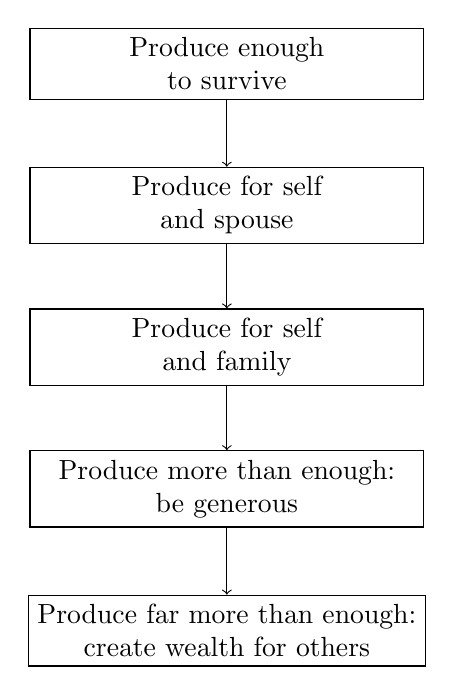
\begin{tikzpicture}[x=1cm,y=1cm]
\node[draw, rectangle, align=center, minimum width=5.0cm, minimum height=0.8cm] (a) at (0,0) {Produce enough\\to survive};
\node[draw, rectangle, align=center, minimum width=5.0cm, minimum height=0.8cm] (b) at (0,-1.8) {Produce for self\\and spouse};
\node[draw, rectangle, align=center, minimum width=5.0cm, minimum height=0.8cm] (c) at (0,-3.6) {Produce for self\\and family};
\node[draw, rectangle, align=center, minimum width=5.0cm, minimum height=0.8cm] (d) at (0,-5.4) {Produce more than enough:\\be generous};
\node[draw, rectangle, align=center, minimum width=5.0cm, minimum height=0.8cm] (e) at (0,-7.2) {Produce far more than enough:\\create wealth for others};
\draw[->] (a) -- (b);
\draw[->] (b) -- (c);
\draw[->] (c) -- (d);
\draw[->] (d) -- (e);
\end{tikzpicture}
\caption{Transcript-derived productivity ladder. The lecture treats widening provision as a rise into a higher kind of life, not merely as a larger income.}
\end{figure}

\subsection{Question \& Answer}

\paragraph{Question.} Why produce more than we need for ourselves and our family?

\paragraph{Answer.} Because for Rohn survival is only the beginning. A solitary survival life is possible, but it is not yet the richer life he is describing. The moment provision exceeds mere need, generosity becomes possible; beyond that, support of worthy projects becomes possible; beyond that, the creation of wealth for others becomes possible. The economic ladder becomes an ethical ladder.

Rohn makes the point with a worked example. If yearly production is
\begin{align}
P &= \$10\,\text{million},
\end{align}
and yearly family need is
\begin{align}
N &= \$3\,\text{million},
\end{align}
then the surplus is
\begin{align}
S &= P-N = \$7\,\text{million}.
\end{align}
The lecture's interpretation of \(S\) is crucial. This is not introduced as private luxury. It is introduced as giving capacity: \(\$7\) million now available to support, endow, and enlarge.

Rohn then pushes one rung further, through the Mark Hughes example. Here the concrete figures matter because the speaker uses them to dramatize a business imagination larger than self-maintenance:
\begin{align}
V_{\mathrm{company}} &\approx \$680\,\text{million}, \\
L_{\mathrm{son}} &\approx \$350\,\text{million}, \\
W_{\mathrm{others}} &\approx \$3.5\,\text{billion}.
\end{align}
The point is not financial analysis. The point is that economic life may be ordered so as to create wealth outwardly, not merely inwardly.

Someone in the lecture asks, why do that? Rohn's answer is short and telling: why not? The ladder is open. Ordinary life is permissible. Extraordinary life is better.

\section{Multiple Skills, Old Fundamentals, Ratios, and the 80--20 Rule}

After this wide imaginative expansion, the lecture narrows itself on purpose. Rohn returns to method. If we are to take advantage of the century, we should learn multiple skills and more than one language. His practical argument is simple: the person who can translate across boundaries is uniquely valuable.

This is why he insists that a child can learn as many languages as one will teach. He even warns against letting a child develop only \(10\%\) or \(15\%\) of what he is capable of. The transition from here to fundamentals is important. The lecture does not want variety of skill to become a search for novelty. It wants variety of skill built on a few enduring truths.

Rohn therefore says that fundamentals are just a few, and that truth is old. The phrase is memorable because it pushes against the appetite for gimmicks. Fundamentals are like antiques, not inventions.

The first explicit law in this part of the lecture is the law of averages. The speaker gives it verbally: if we do something often enough, we will soon have a ratio of results. As editorial shorthand only, we may write
\begin{equation}
R=\frac{s}{n},
\end{equation}
where \(n\) is the number of attempts and \(s\) is the number of successful outcomes. The lecture's own example is plain:
\begin{align}
R_1 &= \frac{1}{10}, \\
R_2 &= \frac{2}{10}.
\end{align}
That second ratio does not appear because the law changed. It appears because the person changed. ``Talk to ten more, get another one'' becomes ``talk to ten more, get two instead of one'' because skill improves.

The second law is the 80--20 rule:
\begin{equation}
20\%\text{ of the people do }80\%, \qquad 80\%\text{ do }20\%.
\end{equation}
Rohn then gives a time-management corollary:
\begin{equation}
t_{20}=80\%\text{ of }T, \qquad t_{80}=20\%\text{ of }T.
\end{equation}
Here \(T\) is available time, \(t_{20}\) is time given to the productive \(20\%\), and \(t_{80}\) is time given to the remaining \(80\%\). He even applies this to the products brought to seminars: stock for the \(20\%\), not for everyone indiscriminately.

\subsection{Question \& Answer}

\paragraph{Question.} Why does the same presentation produce sharply different reactions?

\paragraph{Answer.} Because human response is itself distributed. The lecture offers categories rather than a theorem: laughers, mockers, the confused, and believers. The sameness of the presentation does not imply sameness of reception. That is why ratio-thinking matters.

The Peter example sharpens the point. Out of a large audience, the number who believed is said to be about
\begin{equation}
\text{believers} \approx 3000.
\end{equation}
The lecture does not give the total. It does not need to. The point is that once we understand the lawfulness of uneven response, we stop being surprised by it and begin to work intelligently within it.

Having come back to a few old laws, the lecture is ready to return to its master word: philosophy.

\section{Personal Philosophy as Guidance System and Learning Regimen}

Rohn now says directly what has been implicit from the beginning: each person's personal philosophy is the greatest determining factor in how life works out. That sentence gathers together the opening economic example, the income ladder, the self-development rule, the language section, the productivity ladder, and the ratio laws. Philosophy is the hidden cause that makes those outward results hang together.

He briefly illustrates this with political economy. The communist philosophy, as he describes it, says that capital belongs to the state, not the people. The American counter-philosophy says that capital belongs to the people, not the state. The consequences, he says, are immense. His numerical emblem is East Germany:
\begin{align}
\text{cleanup cost} &\approx \$1\,\text{trillion} \\
&= \$500\,\text{billion already spent} + \$500\,\text{billion still to go}.
\end{align}
Again, the number is not developed analytically. It stands as a lecture-given sign that philosophy has large material consequences.

\begin{definition}
A \emph{personal philosophy}, in the operational sense of this lecture, is a guidance system.
\end{definition}

The guidance system has two main functions:
\begin{equation}
\text{dangers} \to \text{minimize}, \qquad
\text{opportunities} \to \text{maximize}.
\end{equation}

\begin{figure}[t]
\centering
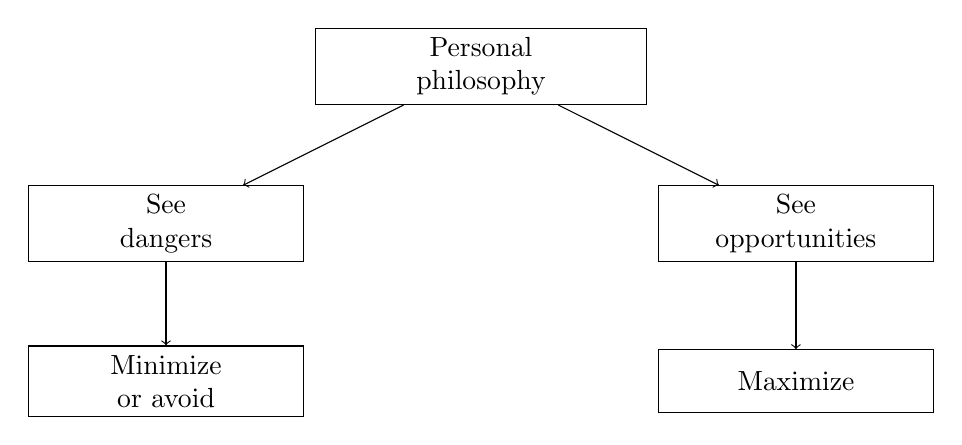
\begin{tikzpicture}[x=1cm,y=1cm]
\node[draw, rectangle, align=center, minimum width=4.2cm, minimum height=0.9cm] (c) at (0,0) {Personal\\philosophy};
\node[draw, rectangle, align=center, minimum width=3.5cm, minimum height=0.8cm] (d1) at (-4.0,-2.0) {See\\dangers};
\node[draw, rectangle, align=center, minimum width=3.5cm, minimum height=0.8cm] (d2) at (-4.0,-4.0) {Minimize\\or avoid};
\node[draw, rectangle, align=center, minimum width=3.5cm, minimum height=0.8cm] (o1) at (4.0,-2.0) {See\\opportunities};
\node[draw, rectangle, align=center, minimum width=3.5cm, minimum height=0.8cm] (o2) at (4.0,-4.0) {Maximize};
\draw[->] (c) -- (d1);
\draw[->] (d1) -- (d2);
\draw[->] (c) -- (o1);
\draw[->] (o1) -- (o2);
\end{tikzpicture}
\caption{Transcript-derived reconstruction of Rohn's ``guidance system.'' The point is not formal optimization but disciplined navigation.}
\end{figure}

As a compact note-writer summary only, one may write
\begin{equation}
\text{good life} \sim \min(\text{dangers})+\max(\text{opportunities}).
\end{equation}
But the lecture itself now pauses to ask the deeper question.

\subsection{Question \& Answer}

\paragraph{Question.} Why is life both danger and opportunity?

\paragraph{Answer.} Here Rohn does not give a proof; he gives a storyteller's answer. Repeatedly he says, ``it seems like.'' It seems like God wished to create a great adventure for the humans he made. The long narration about Lucifer, insurrection, Job, wager, loss, and fidelity is not there as doctrinal system. It is there to preserve one structural intuition: danger is not a temporary mistake in reality. It belongs to the very adventure within which opportunity becomes meaningful.

Once this theological stretch has done its work, the lecture turns back to practice. If life is built this way, then we must learn. We learn from what we see, from what we hear, and from what we read:
\begin{equation}
\text{sight}, \qquad \text{hearing}, \qquad \text{reading}.
\end{equation}
This is the learning triad that closes the lecture's large arc. We pay attention. We return to assemblies. We listen again. We read the books we need to read. We become selective listeners. And, in one of the lecture's finest closing lines, we stand guard at the door of the mind.

The chapter then circles all the way back to economics. Rohn even gives a child's-scale image of capitalism: two bicycles, one to ride and one to rent. That is how simple the intuition of profit may begin. The lecture's final compression is therefore exactly the one with which it ought to close:
\begin{equation}
\text{wages} \to \text{a living}, \qquad
\text{profits} \to \text{a fortune}.
\end{equation}
He states it in plain English as well: profits are better than wages. The circle is complete. The talk began with the difficulty of changing wages and ends with a broader philosophy of profit, learning, and self-directed increase.

\section{Summary}

Rohn's lecture unfolds in a strict order, and that order is its argument. We begin with a low wage and the failure of three weak philosophies. We then learn to ask the repeated tenfold question, not because arithmetic itself is profound, but because it trains the sense of possibility. The lecture then supplies the hinge: work harder on yourself than on your job. From there success becomes attraction, the extraordinary life becomes imaginable, the new century is described as open but competitive, words become a form of capital, fruitfulness becomes productivity, surplus becomes generosity, fundamentals become ratio laws, and philosophy becomes a guidance system for danger and opportunity.

The very end matters because it closes the loop. After all the widening motions of the chapter, we come back to the simplest economic distinction, now transformed by everything in between: wages make a living; profits make a fortune. That sentence is no longer a slogan at the end of the lecture. It is the final consequence of the whole structure we have been led through step by step.